\documentclass{bioinfo}

%\usepackage{graphicx}
%\usepackage{color}
%\usepackage{amssymb}
%\usepackage{amsmath}
%\usepackage{multirow}
%\usepackage{multicol}
%\usepackage{array}
%\usepackage{rotating,capt-of}
%\usepackage{caption}
%\captionsetup[table]{skip=10pt}
%\usepackage{booktabs}
%\usepackage{float} 
%\usepackage{afterpage}
%\usepackage{epsfig} %, a4wide}

%\newcommand{\myparagraph}[1]{
%  \paragraph*{\normalfont\itshape #1}\hspace{5pt}}
%
%\renewcommand\dblfloatpagefraction{0.03}
%\renewcommand\topfraction{.95}
%\renewcommand\bottomfraction{.95}
%\renewcommand\textfraction{.05}
%\renewcommand\floatpagefraction{.95}
%\renewcommand\dbltopfraction{.95}
%\renewcommand\dblfloatpagefraction{.95}



\newcommand{\TODO}[1] {\begingroup\color{red}#1\endgroup}
\newcommand{\SC}[1] {\begingroup\color{purple}#1\endgroup}
\newcommand{\ACC}[1]{\emph{\textbf{#1}}}
\newcommand{\s}[1]{\begin{tiny}#1\end{tiny}}
\newcommand{\url}[1]{\texttt{https://\small #1}}
\newcommand{\maxentscan}{\texttt{MaxEntScan}}
\newcommand{\NEW}[1]{\begingroup\color{black}#1\endgroup}

%% programs
\newcommand{\spps}{\texttt{SPPS}}
\newcommand{\tri}{\texttt{TRI\_tool}}
\newcommand{\lr}{\texttt{LR\_PPI}}

%% databases
\newcommand{\ncbi}{\texttt{NCBI}}
\newcommand{\nega}{\texttt{Negatome Database}}
\newcommand{\kups}{\texttt{KUPS}}

\newcommand{\tool}{\textsc{ProteinPrompt}}

\copyrightyear{2018}
\pubyear{2018}
\access{Advance Access Publication Date: Day Month Year}
\appnotes{Protein-Protein-Interaction, Machine Learning, Random Forest}


\begin{document}
\firstpage{1}

\subtitle{Structural Biology}

\title{\tool: fast and accurate prediction of protein-protein-interactions}

\author{Sebastian Canzler$^{\text{\sfb 1,3,4,} *}$, Ren\'{e} Staritzbichler$^{\text{\sfb 1,2,} *}$}

\address{
  $^{\text{\sf 1}}$Immuthera GmbH, L{\"o}{\ss}niger Stra{\ss}e 16, 04275 Leipzig, Germany and 
  $^{\text{\sf 2}}$Bioinformatics Group, Department of Computer Science, University of Leipzig, H{\"a}rtelstra{\ss}e 16-18, 04107 Leipzig, Germany and
  $^{\text{\sf 3}}$ProteinFormatics Group, Institute of Medical Physics and Biophysics, University of Leipzig, H{\"a}rtelstra{\ss}e 16-18, 04107 Leipzig, Germany and
  $^{\text{\sf 4}}$Young Investigators Group Bioinformatics and Transcriptomics, Department of Proteomics, Helmholtz Centre for Environmental Research - UFZ, 04318 Leipzig, Germany.}


\corresp{$^\ast$To whom correspondence should be addressed.}

\history{Received on XXXXX; revised on XXXXX; accepted on XXXXX}

\editor{Associate Editor: XXXXXXX}


\abstract{\textbf{Motivation:}  Protein-protein interactions are among the key drivers of biology and thus are an important class of targets for medical regulation.
  Here, we present \tool, a precise machine learning method for the calculation of protein-protein interactions.
  Learning methods depend crucially on both size and quality of datasets used for training and testing.
  Starting point of \tool\  was therefore the collection of a comprehensive dataset from basically all available sources.
  In turn, a very thorough filtering was imperative.
  The actual key step is the transformation of the original sequence data into a representation that enables the learning algorithm to understand the underlying patterns that lead to binding versus non-binding.
  \tool\  exploits the random forest algorithm using auto-correlation of seven amino acid scales.\\
  \textbf{Results:}
  Based on this combination, \tool\  is reaching an area under curve of 0.95, which is far above any other publicly available tool. \\
  \textbf{Contact:} \href{rene.staritzbichler@medizin.uni-leipzig.de}{rene.staritzbichler@medizin.uni-leipzig.de}, \href{sebastian@bioinf.uni-leipzig.de}{sebastian@bioinf.uni-leipzig.de} }


\maketitle




\section{Introduction}

Interacting proteins are among the key players of biology. The driving
force of molecular networks are protein interactions rather than
single protein components, accomplishing their individual functions
\citep{Pawson:2004}. Biological processes, such as cellular
organization, communication, regulation of transcription and
translation, or immune responses require various proteins to interact
and work together to function appropriately. The experimental
identification of interacting proteins is highly expensive and time
consuming.

Many biochemical and biophysical methods for research and medical diagnostics are based on protein-binding:
ELISA,
gel electrophoresis, immunoblot, florescence anisotropy, FRET,
Cross-linking with mass spectrometry. For high-throughput-screening of
large libraries there are techniques such as phage display. 

A reliable \textit{in silico} prediction of protein-protein
interactions (PPI) will therefore shed more light on biological and
pharmacological responses and pathways. Computations may complement
and guide biochemical assays. However, explicit molecular dynamics or
docking approaches require structural detail, which is often out of
reach. Even if structural knowledge is available, these methods are
computational highly expensive and therefore are not applicable for
scanning libraries of candidates. 

Both when structural insight is lacking and when speed is crucial,
other methods need to be applied. \TODO{Non structure-based (or Non-structure-based? or without a hyphen?)} computational
approaches of identifying potential PPIs are generally based on an
extensive set of known protein-protein interactions, information about
cellular localization, amino acid sequences, or secondary structures.

Such methods may include phylogenetic trees \citep{Pazos:2001},
phylogenetic profiles \citep{Barker:2005}, network-based methods
\citep{Yook:2004, Clauset:2008}. In recent years, the more
sophisticated approach of combining distinct prediction methods has
been applied, e.g., \texttt{STRING} \citep{Szklarczyk:2011} or
\texttt{PIPS} \citep{McDowall:2009}.

Nevertheless, different proteome-wide prediction methods have shown
that knowledge of the amino acid sequence alone may be sufficient to
identify novel, functional protein-protein interactions
\citep{Martin:2005, Shen:2007}.
Mostly, these methods rely on statistical learning algorithms.
Due to its prominent and major advantages like simplicity, rapidity, and generality, this kind of
prediction method became increasingly widespread over the last years
\citep{Ofran:2003, Betel:2007, Liu:2012, Perovic:2017, Pan:2010}.
Overall, biology has seen a massive raise in applications
of artificial intelligence and deep learning in the recent years
\citep{Ching:2018}.

In this paper, we present a sequence-based method for predicting
PPIs that outperforms all other currently available methods distinctively.
The predictive power was boosted by a rigorous fine-tuning
of the machine learning key elements, such as
dataset generation and the design of the feature vector.
Auto-correlation of hydrophobicities,
in conjunction with a random forest (RF) machine learning algorithm,
has lead to maximum accuracy.
Additionally to its outstanding quality, it is 
an extremely fast high-throughput
method.

Therefore, \tool\  (\textbf{protein} \textbf{pr}ediction \textbf{o}f \textbf{m}atching \textbf{p}ar\textbf{t}ners)
may serve as a reliable method for identifying potential interaction partners from a database of
known proteins, and may thus help to identify the yet unknown
biological role of many proteins.


\section{Materials and Methods}

To maximize the predictive power, it is pivotal to optimize each of
the key elements, i.e., the calculation of the feature vector, the
collection of the training and testing data, and finally, the
selection and fine-tuning of the machine learning algorithm. 

For all aspects, many variations were tested. Here we focus on the
ones leading to the highest accuracy. 


\subsection{Feature vector calculation}
The feature vector calculation includes the extraction and
transformation of sequence-based information into a numerical vector
of constant size. Therefore, it is crucial to extract the properties
that are responsible for directing the protein-protein interaction. 

Each amino acid sequence of a protein-protein complex was transformed
into a sequence of numerical values representing seven
sequence-derived physicochemical properties, which include
hydrophobicity \citep{Eisenberg:1984, Koehler:2009}, hydropyhilicity
\citep{Hopp:1981}, volumes of side chains of amino acids
\citep{Krigbaum:1979}, polarity \citep{Grantham:1974}, polarizability
\citep{Charton:1982}, solvent-accessible surface area \citep{Rose:1985}
and net charge index of side chains of amino acids \citep{Zhou:2006}
for each residue in the sequence. These scales are commonly applied in
protein interaction prediction \citep{Bock:2001, Bock:2003},
alignment \citep{Stamm:2013}, protein recognition \citep{Ding:2001},
protein structure prediction \citep{Durham:2009}, or the prediction of
protein functional families \citep{Cai:2003}. These applications
suggest that these properties significantly contribute to the
stability of the protein-protein complexes. Each of these amino acid
scales was normalized as follows: 

\begin{equation}
P'_{i} = (P_i - \overline{P}) / \sigma_P
\end{equation}

where $\overline{P}$ is the mean and $\sigma$ is the standard
deviation of the scale-based descriptor covering 20 amino acids,
respectively: 

\begin{equation}
\overline{P} = \sum^{20}_{i=1}P_i / 20
\end{equation}
 and 
\begin{equation}
\sigma_P = \sqrt{\frac{1}{20} \sum^{20}_{i=1}(P_i - \overline{P})^2}
\end{equation}

The subsequent transformation into suitable feature vectors using
auto-correlation (AC) works as follows: 

\begin{equation}
AC_{lag, j} = \frac {\frac{1}{n-lag} \sum^{n-lag}_{i=1} ( S_{i,j} - \overline{S_j}) (S_{i+lag,j} - \overline{S_j})} { \sigma_{S_j} * \sigma_{S_j} }
\end{equation}
where $S_j$ is the translated amino acid sequence using the normalized
scale-based descriptor $P'_j$ with $j = 1, 2, \dots, 7$ , $n$ is the
length of sequence S, and $lag = 1, 2, \dots, 30$  being the shift for
which the auto-correlation is being calculated. $\overline{S_j}$ and
$\sigma_{S_j}$ are the mean and standard deviation of the translated
sequence, respectively. \citet{Ding:2016} showed that a maximal
$lag$ of less than 30 tends to lose useful information while the
larger values may induce noise. 

The number of AC values for each of the seven scales is 30. 
The feature vector describing any individual amino acid sequence has 210 elements or dimensions.
Thus, for a pair of sequences, the feature space has 420 dimensions. 


\subsection{Collecting data-points}
In order to create comprehensive training and testing data we tried to
collect as many trustworthy PPI annotations as possible. We included
data from various sources such as \texttt{Database of Human
  Interacting Proteins}\footnote{http://dip.doe-mbi.ucla.edu/} (DIP)
\citep{Salwinski:2004}, \texttt{Human Protein Reference
  Database}\footnote{http://www.hprd.org/} (HPRD)
\citep{Keshava_Prasad:2009}, \texttt{Protein
  Database}\footnote{www.rcsb.org} (PDB) \citep{Berman:2000}, and the
\nega\footnote{http://mips.helmholtz-muenchen.de/proj/ppi/negatome/}
\citep{Blohm:2014}. We also included annotations retrieved from the
\kups \footnote{http://www.ittc.ku.edu/chenlab/kups/}   server
\citep{Chen:2011} which mainly incorporates PPIs from
\texttt{MINT}\footnote{https://mint.bio.uniroma2.it/}
\citep{Licata:2012} and
\texttt{IntAct}\footnote{https://www.ebi.ac.uk/intact/}
\citep{Orchard:2014}. In addition to the negative annotations collected
from the \nega, the \kups\ server generated negative data-points based
on the the following criteria: (1) proteins should be functional
dissimilar, (2) proteins should be localized in different cellular
compartments, and (3) proteins are part of non-interacting domains. 

After intense manual curation and mapping of different names describing
the exact same protein, we derived a total amount of 31,867 distinct
human proteins. For this set, 73,681 positive PPIs were collected
from the datasources previously mentioned. By means of \texttt{CD-hit}
\citep{Li:2006, Fu:2012}, we reduced this set to 41,844 positive
protein-protein pairs with at most 50\% sequence identity. For
negative pairs, we collected over 1.5 million unique protein-protein
pairs, from which we randomly selected a number of PPIs, that was
matching the size of the positive dataset.

Finally, our training dataset contains 36,750 positive and 36,750
negative PPIs, while our testing dataset contains 5094 positive and
5094 negative data-points.
The separation into test and training data is required to counterbalance overfitting.
While the actual learning is performed on the training data,
the simultaneous monitoring of the test data allows to determine the point where overfitting starts.
Overfitting begins when the prediction quality for the test data is starting to decrease,
while it is still improving for the training data.

For further enhancement of the prediction
quality of \tool, we also incorporated inverse and reverse PPI
representations. Each protein-protein pair $AB$ is described in the
original and inverse direction ($A$: ``ABC'' $\rightarrow$ $A'$:  ``CBA''),
as well as in original and reversed order ($AB$,$BA$).
In the final dataset each annotated PPI is represented
in four distinct descriptions. Example pseudo-sequences: (``ABCD'', ``KLMN''),
  (``ABCD'', ``NMLK''), (``KLMN'', ``ABCD''), (``KLMN'', ``DCBA'')

To assess the prediction quality of \tool, we compared our method to
several other publicly available programs. As some of them are limited
in speed or upload capacity to their webserver, it was not
feasible to perform this test using our entire test dataset with more
than 10k datapoints. Instead, we randomly selected 495 positive and 473
negative pairs from our test set.


\subsection{Selection of learning method}
Many implementations of various learning algorithms are
available. By means of the \texttt{caret} R package \citep{Kuhn:2008},
the fine-tuning and comparison is relatively easy. We tested several
artificial neural network implementations, support vector machines and
tree-based methods. After identifying the random forest approach as
performing best on our extensive testing and training datasets,
we moved to a Python-based implementation mainly
due to speed reasons.  


\subsection{Random forest classification}
Random forest (RF) is an algorithm, which uses an ensemble of
classification trees \citep{Breiman:2001}. Each classification tree is built by using a
bootstrap sample of training data, and each split candidate set is a
random subset of variables. RF uses both bagging (bootstrap
aggregation) and random variable selection for tree building. Each
classification tree is unpruned to obtain low-bias trees. The bagging
and random variable selection can cause low correlation of individual
trees. Therefore, RF has excellent performance in classification
tasks. 

We define a 420-dimensional feature vector $F=(x_1,x_2,
\dots,x_{420}$) as the input data of RF model. If the number of cases
in the training set is $N$, the sample is built by randomly choosing
$N$ cases from the original data, but with replacement. This sample
will be the training set for growing the tree. There are $M$ input
variables, a number $m \ll M$ is specified such that at each node, $m$
variables are selected at random out of $M$ and the best split on
these m is used to split the node. The value of $m$ is held constant
during the forest growing. Each tree is grown to the largest extent
possible without pruning. The final number of trees in the forest is
set to 750 due to run-time optimization. 




\section{Results}


\subsection{Performance}
\label{performance}

Based on our test set of 5094 positive and 5094 negative cases
(binders vs. non-binders), we plot the receiver operation
characteristics (ROC) curve, see Figure \ref{fig:roc}.
These allow not only to estimate the overall quality of the predictions, but also
gives a visual overview over the relationship between true and false
positives.
Every point on the curve shows how many falsely predicted binders one has to expect for how many correctly predicted ones.
As the datapoints are sorted by their predicted binding propensity, a reasonable threshold can be selected.
This allows for a finetuning of the balance between sensitivity versus specificity.

Sensitivity is the ratio of correctly predicted binders (true positives), to actual binders.
  Specificity is then the ratio of correctly predicted non-binders (true negatives) to all non-binders.
  For example, in Figure \ref{fig:roc} a false positive rate of 0.03 will lead to a true positive rate of $\sim$0.6.
  Thus, selecting this point (its associated score) as threshold will give a hit rate of 60\%, while only 3\% false predictions have to be expected.


An ideal signal would lead to a plot with rectangular shape
with an area under the curve (AUC) of 1. The other extreme, pure noise, would be a diagonal
line with an AUC of 0.5.

Our method reaches an AUC of 0.95,
specificity: 0.88,
sensitivity: 0.87,
accuracy: 0.88.

Currently, our method balances specificity and sensitivity to avoid an
unwanted bias in different applications.

\begin{figure}[t]
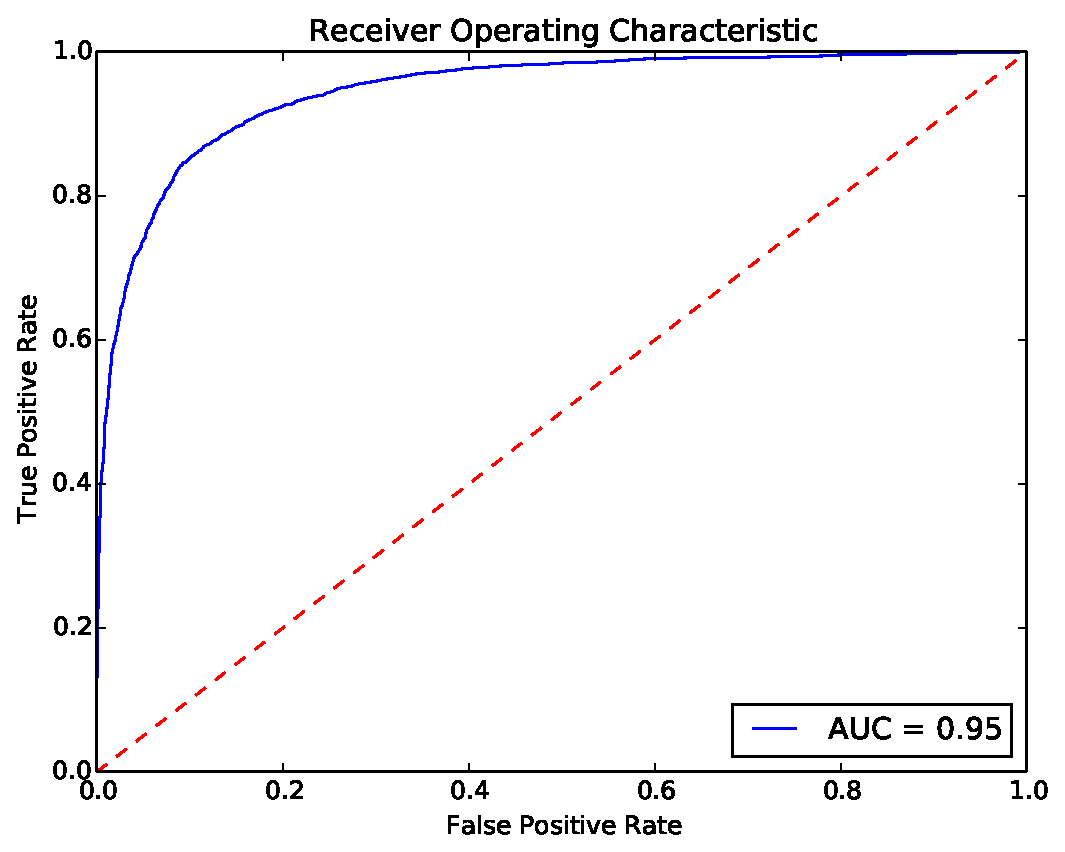
\includegraphics[width=0.5\textwidth]{img/meta_final_roc.eps}
\caption{Performance of \tool\  tested on the whole test dataset
  containing over 10,000 PPIs.}
\label{fig:roc}
\end{figure} 



\subsection{Comparison to other tools}

To verify our achievements, we compared our program against publicly
available tools such as \spps\ \citep{Liu:2012}, \tri\
\citep{Perovic:2017}, and \lr\ \citep{Pan:2010}. Therefore, we used the
diminished test dataset, as described in the Methods section. 

Since we re-evaluated \tool\  on the dimished testset, to ensure
comparability, the results are somewhat different compared to the
whole testing data set. 

\begin{figure}
  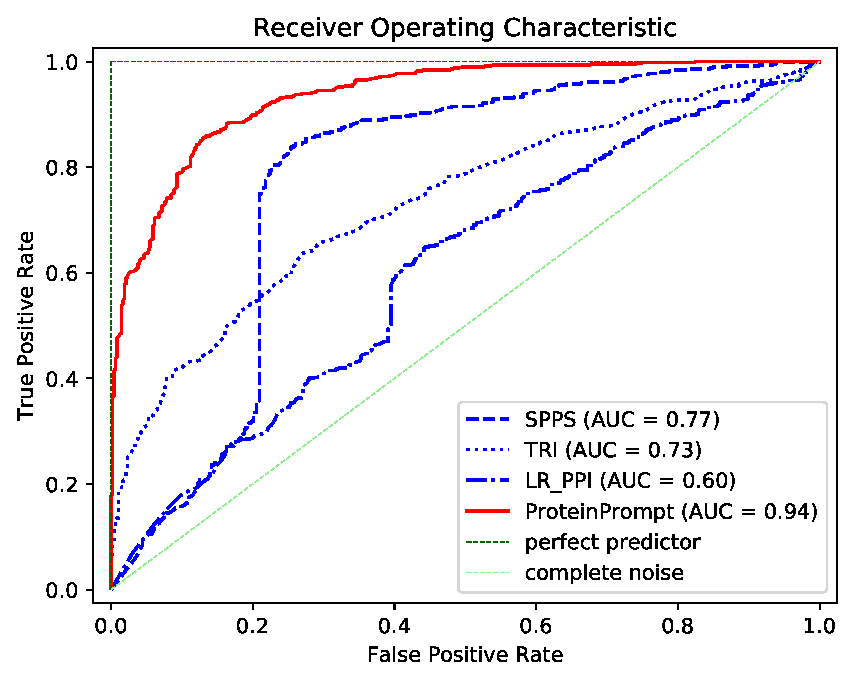
\includegraphics[width=0.5\textwidth]{img/comparison_roc.eps}
  \caption{Comparison of ROC-curves between \tool, \spps, \tri, \lr\ 
    using the diminished test dataset that included 968
    protein-protein pairs.}
  \label{fig:comparison}
\end{figure}


\begin{table}
\begin{tabular}{|l |c | c | c | c |}
  \hline
  Tool  & AUC & Spec. & Sens. & Acc. \\
  \hline
  \tool\   & 0.94 & 0.88 & 0.84 &  0.86 \\
  \hline
  \spps\  & 0.77 & 0.34 & 0.96 & 0.66 \\
  \hline
  \tri\  & 0.73 & 0.95 & 0.32 & 0.63 \\
  \hline
  \lr\  & 0.60 & 0.16 & 0.91 & 0.53  \\
  \hline
\end{tabular}
\caption{ Quality measures of \tool, compared to other publicly
  available tools, such as \spps\ \citep{Liu:2012}, \tri\
  \citep{Perovic:2017}, and \lr\ \citep{Pan:2010}.
  Listed are area under curve (AUC), specificity, sensitivity and accuracy.}
\label{table:comparison}
\end{table}

The results shown in Table \ref{table:comparison} and the ROC plot in
Figure \ref{fig:comparison} suggest that \tool\  clearly outperforms all
three competitors. \tool\  is furthermore the only method that finds a
balance between sensitivity and specificity. \spps\ and \lr\ show an
excellent sensitivity of 0.96 and 0.91, however, their
specificity is rather poor with 0.34 and 0.16, respectively. \tri\ on
the other hand shows a massive bias towards specificity, 0.95 compared
to a sensitivity of 0.32 .
Additionally, the overall prediction accuracy and the area under the curve are significantly higher.
Accuracy: 0.86 versus 0.66 (\spps), 0.63 (\tri).
AUC: 0.53 (\lr) and 0.94 versus 0.77 (\spps), 0.73 (\tri), and 0.60 (\lr), respectively.


\section{Discussion}

The direct comparison with other available tools
proved the outstanding quality of \tool.
Beside its high accurracy, \tool\ is based on a fast random forrest algorithm.
It is thus possible to scan the entire human proteasome within roughly one minute.
This makes \tool\  both the fastest and most accurate method available. 

After an exhaustive optimization of: i) the learning algorithm, ii)
the contact database, and iii) the representation of the binding
sequences, we identified the random forest algorithm using autocorrelation on seven
residue scales as the ideal combination.

The collection of an extensive database with little redundancy was crucial
and required several iterations of manual curation of the test and training datasets.
The diversity posed hard challenges to the learning
- it would have been easy to reach even higher accuracy values by omitting parts of our dataset.
However, this turned \tool\ into a broadly applicable method.

In our next steps we will extend \tool\  to predict also the binding of short peptides to protein receptors, specifically to those of the GPCR family.
We furthermore intend to expand \tool\  towards antibody-protein binding.
Initial tests have shown, that the methods described in this paper are not directly applicable to this important class of protein interactions - which is easily understood, as the antibody binding mode via 3 very short loop segments does not reflect the general protein binding modes, covered currently by \tool. 

Based on our extensive tests, we expect \tool\
to be beneficial for the understanding of complex networks of protein-protein interactions,
which are the basis for a broad range of mechanisms in biology.


\section*{Acknowledgements} 
Johanna Tiemann, Peter Hildebrand, Alexander Vogel and Thorsten Kaiser for proofreading.
The universe for all the cookies.

\section*{Funding}

This work was funded by the S\"achsische Aufbaubank (SAB).

\bibliographystyle{natbib}
\bibliography{ppi_prediction}

\end{document}


